\section{РАЗРАБОТКА БАЗЫ ДАННЫХ}
\subsection{Концептуальная модель}

\textbf{Предметная область} - совокупность объектов,
свойства которых и отношения между которыми рассматриваются в рамках некоторого исследования.

\textbf{Модель предметной области} - некоторая система, адекватно имитирующая
структуру и функционирование исследуемой предметной области.

\textbf{Концептуальная модель} - это структура моделируемой предметной области,
свойств её элементов и причинно-следственных связей, присущих системе и
существенных для достижения цели моделирования.
В рамках этапа концептуального моделирования выделяются основные смысловые единицы (сущности)
предметной области, определяются и описываются связи между ними.

Концептуальная модель ориентирована на потенциальных пользователей базы данных,
так как представляет предметную область на их уровне понимания.
Этот уровень называется системно-независимым или предметно-ориентированным.

\subsubsection{ЛКМ для БП <<Приказ о создании инвентаризационной комиссии>>}

Локальная концептуальная модель
(спроектированнная с помощью ARIS Express)
для бизнес процесса с документом <<Приказ о создании инвентаризационной комиссии>>
изображена на рисунке~\ref{fig:DataModel_DOC_PrikazCozdInventKom}.

\begin{figure}[!h]
    \centering

    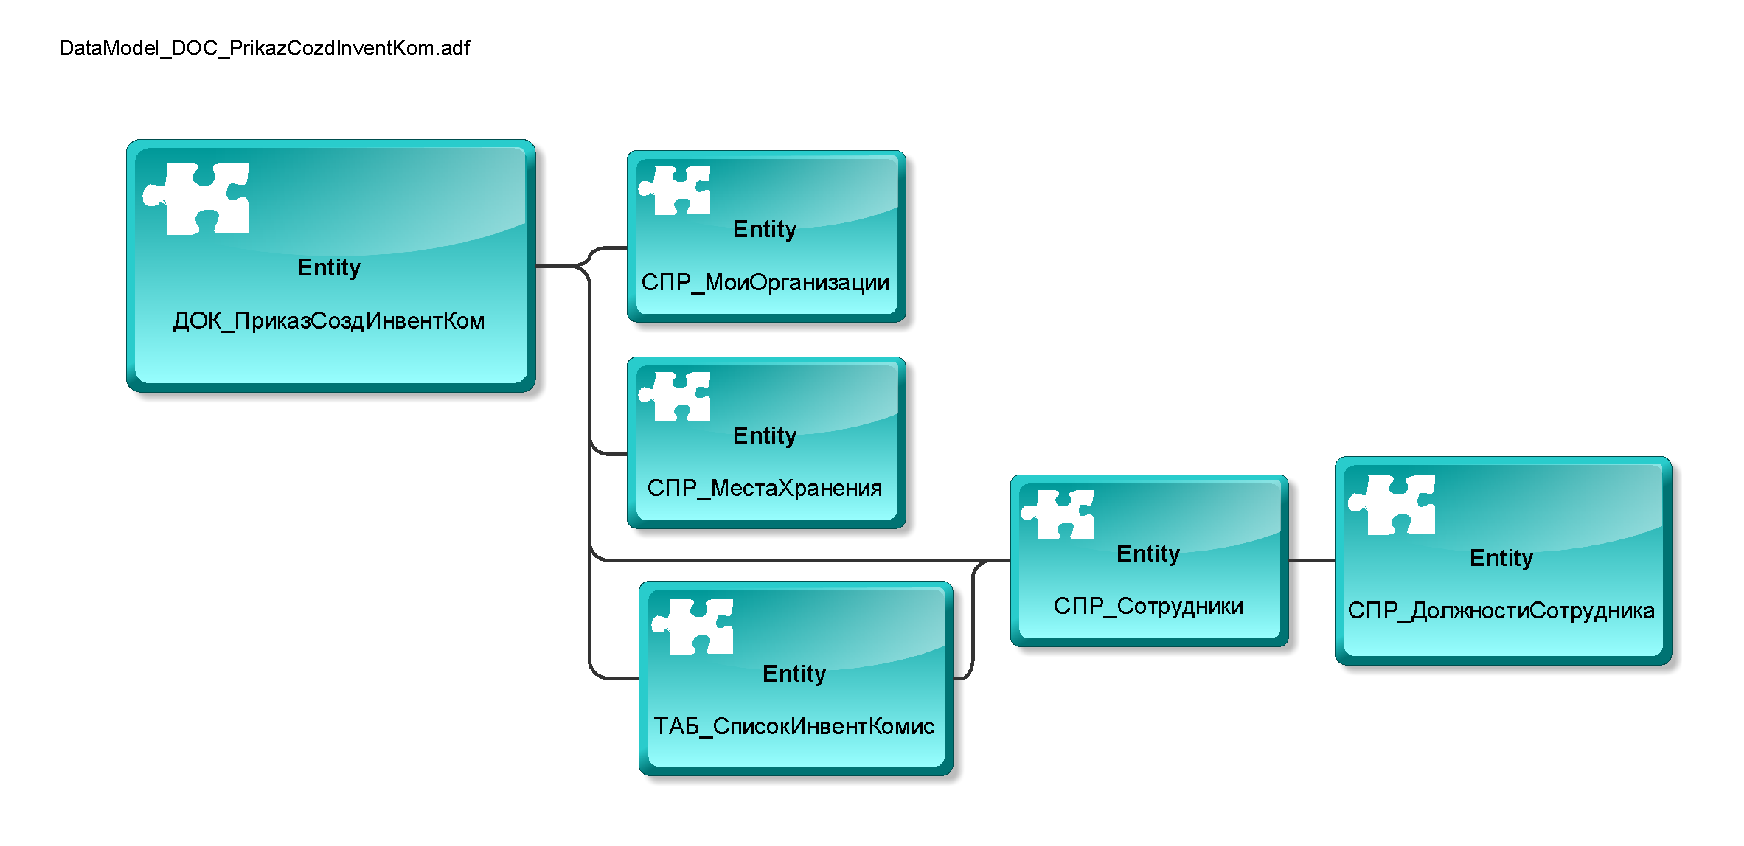
\includegraphics[width=18cm]
    {assets/database/DataModel_DOC_PrikazCozdInventKom.adf.pdf}

    \caption{Локальная концептуальная модель для бизнес процесса с документом <<Приказ о создании инвентаризационной комиссии>>}

    \label{fig:DataModel_DOC_PrikazCozdInventKom}
\end{figure}

\newpage

\subsubsection{ЛКМ для БП <<Инвентаризационная опись>>}

Локальная концептуальная модель
(спроектированнная с помощью ARIS Express)
для бизнес процесса с документом <<Инвентаризационная опись>>
изображена на рисунке~\ref{fig:DataModel_DOC_InventOpic}.

\begin{figure}[!h]
    \centering

    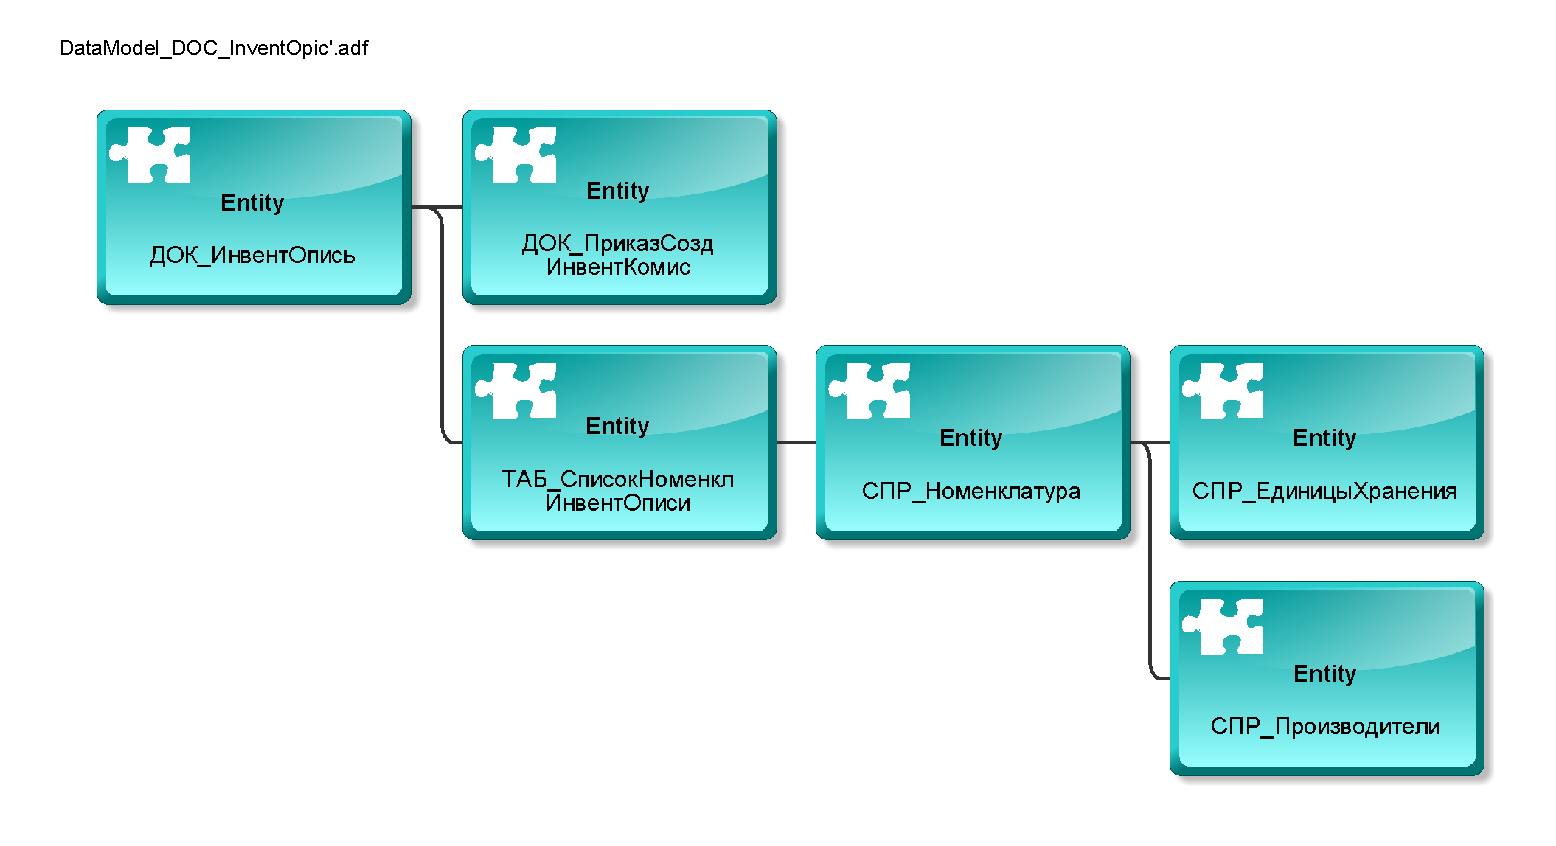
\includegraphics[height=8cm]
    {assets/database/DataModel_DOC_InventOpic'.adf.pdf}

    \caption{Локальная концептуальная модель для бизнес процесса с документом <<Инвентаризационная опись>>}

    \label{fig:DataModel_DOC_InventOpic}
\end{figure}

% \newpage
\subsubsection{КМ для БП ОА}

Концептуальная модель
(спроектированнная с помощью ARIS Express)
для бизнес-процесса объекта автоматизации <<Инвентаризация>>
изображена на рисунке~\ref{fig:DataModel_DOC}.

\begin{figure}[!h]
    \centering
    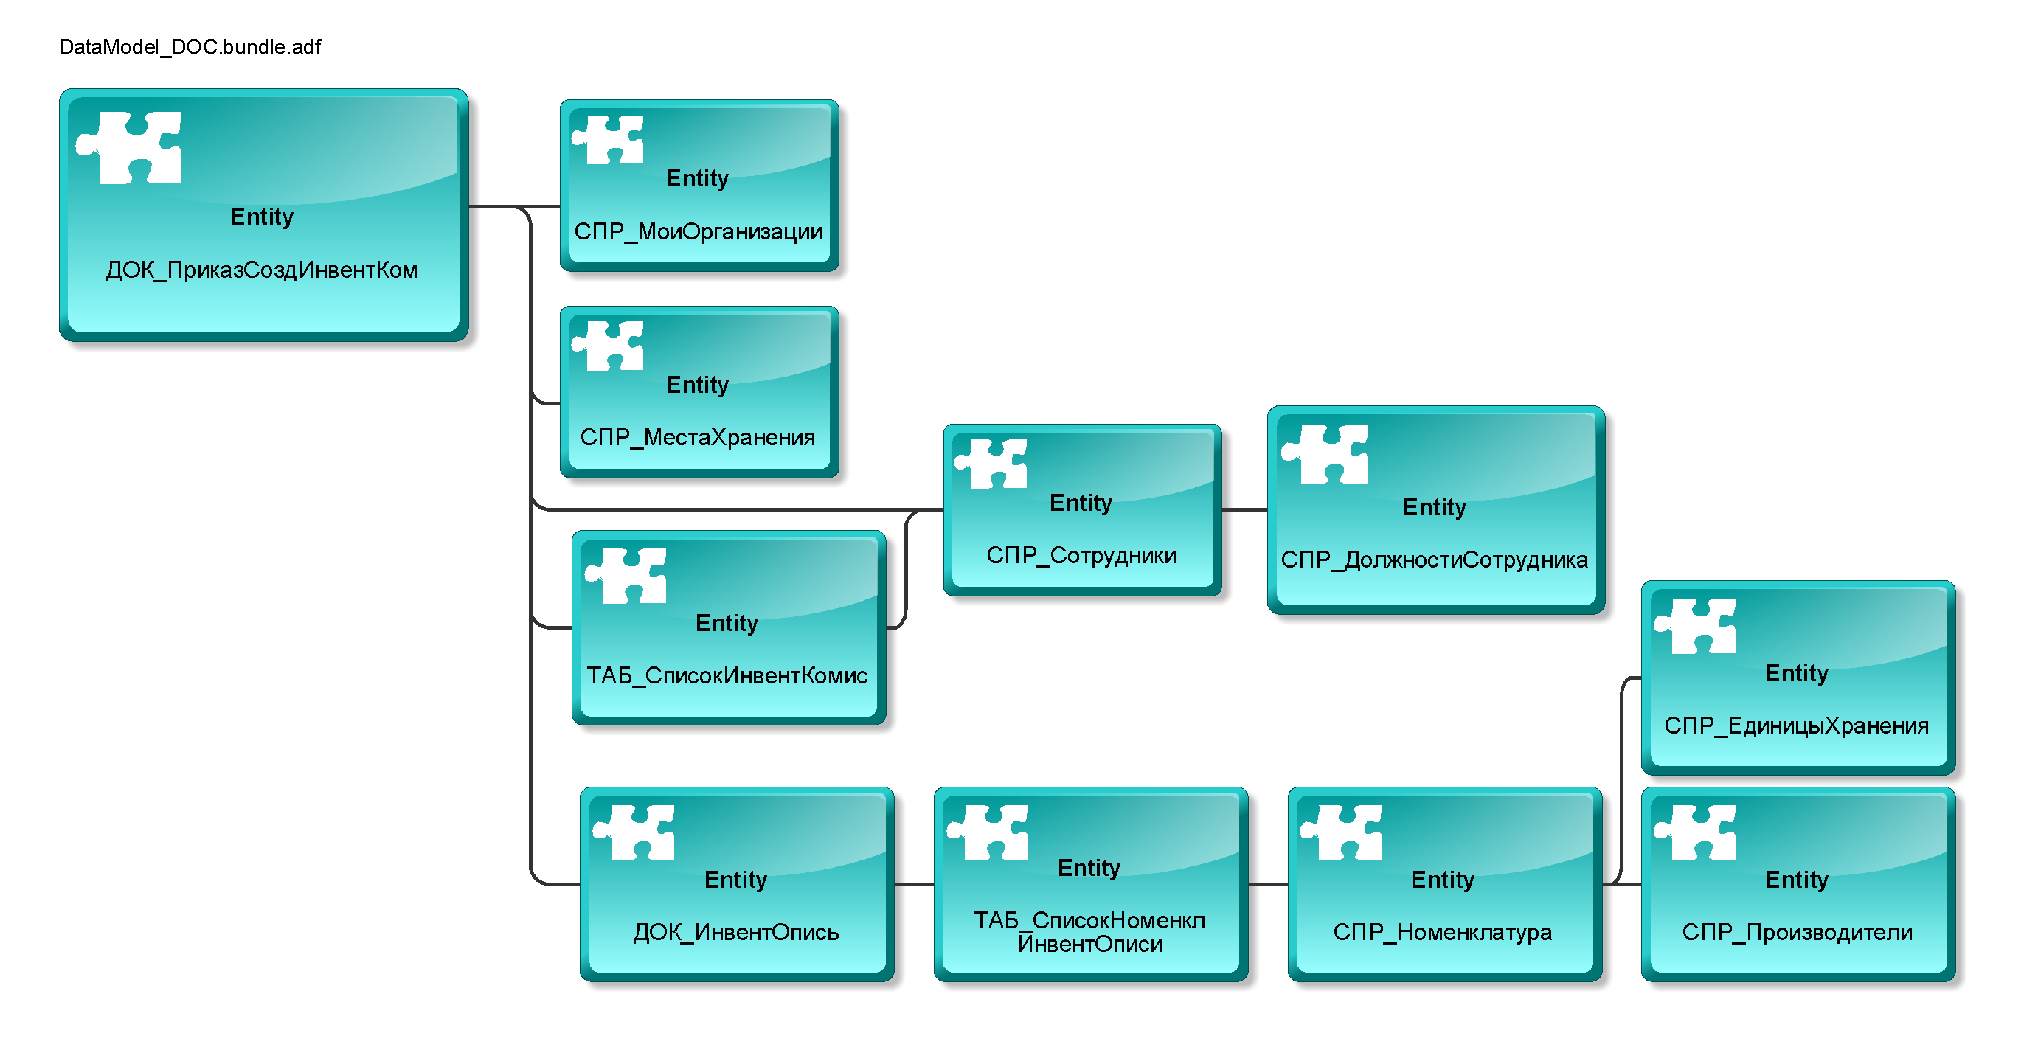
\includegraphics[height=8cm]
        {assets/database/DataModel_DOC.bundle.adf.pdf}
    \caption{Концептуальная модель}
    \label{fig:DataModel_DOC}
\end{figure}

\newpage
\subsection{Логическая модель}

Логическая модель 
изображена на рисунке~\ref{fig:ArchitectureDatabase}.

\begin{figure}[!h]
    \centering

    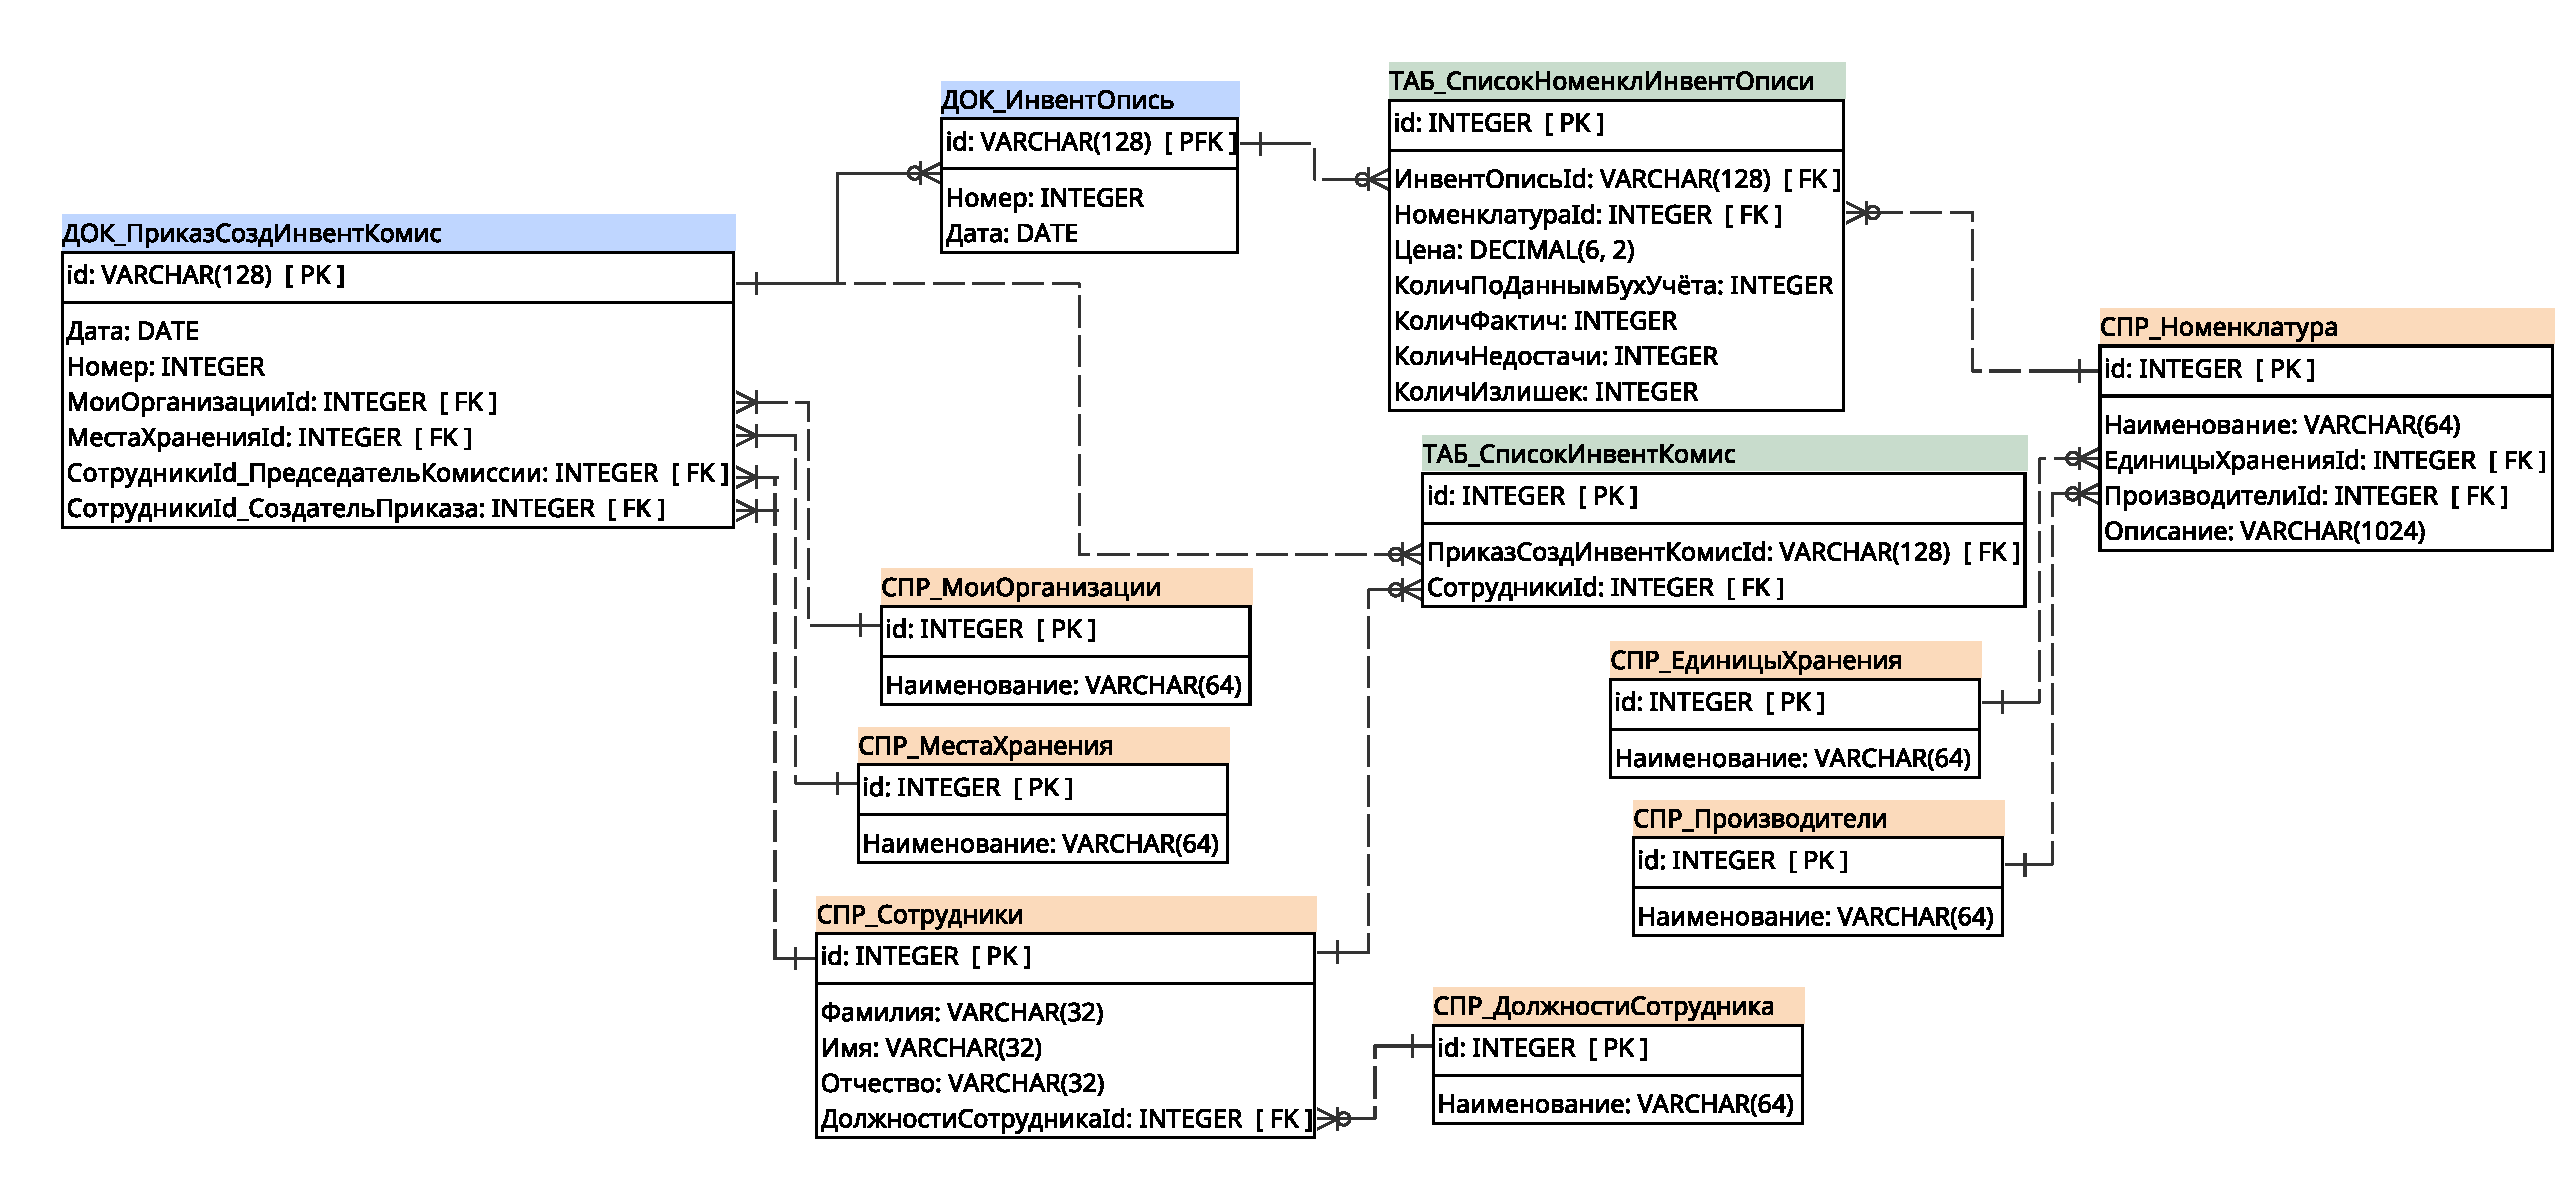
\includegraphics[width=22cm, angle=90]
    {assets/database/ArchitectureDatabase.architect.pdf}

    \caption{Логическая модель}

    \label{fig:ArchitectureDatabase}
\end{figure}

\newpage
\subsection{Физическая модель}

\lstinputlisting[language=sql]
{assets/database/SQL_CreateTable.sql}

\newpage

\lstinputlisting[language=sql]
{assets/database/SQL_DropTable.sql}

\newpage
